\chapter{Brockett-Bedingung für unteraktuiertes mechanisches System}
\label{ch:Brockett_Bedingung_für_unteraktuiertes_mechanisches_System}
In diesem Kapitel wird das berühmte Brockett Theorem vorgestellt. Es ist wie folgend strukturiert: Abschnitt \ref{Mathematische Grundbegriffe} geht es um die Erklärung einiger mathematischen Grundbegriffen, damit die Leser den Beweisvorgang für Brockett-Bedingung leicht verstehen können. Abschnitt \ref{Erläuterung_zur_Brockett-Bedingung} befasst sich mit der Beweisskizze des Theorems.

\section{Mathematische Grundbegriffe}
\label{Mathematische Grundbegriffe}
In Anbetracht von der mathematische Beschreibung und dem Beweis für Brockett-Bedingung ist zuerst die Erklärung einiger mathematischen Terme notwendig. 
\begin{Def}   
	\begin{description} 
		\item[Stetigkeit (engl.: continuity)]
		\cite[S. 250]{grosche2003teubner}:~Es sei $a\subseteq M$. Die Funktion $f:M\subseteq\Reals\to\Reals$ ist genau dann im Punkt $a$ stetig, wenn es zu jeder reellen Zahl $\varepsilon>0$ eine reelle Zahl $\delta>0$ gibt, sodass
		$\left | f\left ( x \right )-f\left ( a \right ) \right |< \varepsilon$ für alle $x\subseteq M$ mit $\left | x-a \right |< \delta $ gilt.  
	\end{description}
\end{Def}
\vspace{-0.8em}
D.h. eine stetige Funktion erfüllt die Bedingung: wenn der Abstand zweier Elemente der Definitionsmenge infinitesimal ist, muss der Abstand ihrer entsprechenden Funktionswerte auch infinitesimal sein.
\begin{Def}
	\begin{description}
		\item[Stetige Differenzierbarkeit (engl.: continuously differentiable)]
		\cite[S. 256]{rudin2009analysis}:~Eine differenzierbare Abbildung $\vect{f}:E\subset\Reals^{n}\to \Reals^{m}$ heißt stetig differenzierbar in $E$, wenn ${\vect{f}}'$ eine stetige Abbildung von $E$ in $L\left ( \Reals^{n},\Reals^{m} \right )$ ist, wobei $E$ eine offene Menge und $L\left ( X,Y \right )$ der Raum linearer Abbildungen ist.
	\end{description}
\end{Def}	
\begin{Def}
	\begin{description}
		\item[Klasse $C^{k}$ (engl.: class $C^{k}$)]
		\cite[S. 265]{grosche2003teubner}:~Eine Funktion gehört zur Klasse $C^{k}$, wenn sie auf einer offenen Umgebung des Punktes $p$ stetige Ableitungen bis zur Ordnung $k$ besitzt.
	\end{description}
\end{Def}
\vspace{-0.8em}
Basierend auf der obigen Definition hat eine Funktion aus der Klasse $C^{1}$ immer eine erste Ableitung, die auch stetig ist.
\begin{Def}
	\begin{description}
		\item[Glatte Funktion (engl.: smooth function)]
		\cite[S. 5]{tu2010introduction}:~Ein Synonym für $C^{\infty}$ ist \emph{glatt}.
	\end{description}
\end{Def}
\vspace{-0.8em}
Eine glatte Funktion ist nämlich eine Funktion mit stetigen Ableitungen bis zur unendlichen Ordnung.
\begin{Def}
	\begin{description}
		\item[Surjektiv (engl.: onto)]
		\cite[S. 931]{grosche2003teubner}:~Gegeben sei die Abbildung $f:X \to Y$. Betrachtet die Gleichung $f\left ( x \right )=y$. Wenn die Gleichung für jedes $y\in Y$ eine Lösung $x\in X$ besitzt, d.h. $f\left ( X \right )=Y$, dann heißt $f$ genau dann \emph{surjektiv}.
	\end{description}
\end{Def}
\vspace{-0.8em}
Mit anderen Worten: eine Abbildung ist surjektiv, wenn jedes Element $y$ der Wertemenge $Y$ erreicht werden kann.
\begin{Def}
	\begin{description}
		\item[Häufungspunkt (engl.: limit point)]
		\cite[S. 35]{rudin2009analysis}:~Ein Punkt $p$ ist ein \emph{Häufungspunkt} der Menge $E$, wenn in jeder Umgebung von $p$ ein Punkt $q\in E$ mit $q\neq p$ liegt.
	\end{description}
\end{Def}
\begin{Def}
	\begin{description}
		\item[Abgeschlossene Menge (engl.: closed set)]
		\cite[S. 36]{rudin2009analysis}:~$E$ heißt abgeschlossen, wenn jeder Häufungspunkt von $E$ in $E$ liegt.
	\end{description}
\end{Def}
\begin{Def}
	\begin{description}
		\item[Beschränkte Menge (engl.: bounded set)]
		\cite[S. 36]{rudin2009analysis}:~$E$ ist beschränkt, wenn eine reelle Menge $M$ und ein Punkt $q\in X$ existieren, sodass der Abstand von $(p,q)$ kleiner als $M$ für alle $p\in E$ gilt. $X$ ist hier ein metrischer Raum, dessen Teilmenge $E$ ist.
	\end{description}
\end{Def}
\begin{Def}
	\begin{description}
		\item[Kompakte Menge (engl.: compact set)]\footnote{Um die Leser den Beweis von Brockett Bedingung leicht versteht, wird ein Korollar von Kompakter Menge zitiert. Eine allgemeine Definition davon ist: .}
		\cite[S. 45]{rudin2009analysis}:~ Falls eine Menge $E$ in $\Reals^{k}$ abgeschlossen und beschränkt, dann heißt sie kompakt.
	\end{description}
\end{Def}
\vspace{-0.8em}
Z.B. das Intervall $\left [ 1,2 \right ]$ ist eine kompakte Menge in $\Reals$ mit $1$ und $2$ jeweils dem linken und rechten Häufungspunkt. %Weil $1$ und $2$ gehört zur $E$ und der Abstand jeder beliebigen zwei Elementen in $E$ kleiner als z.B. $2$. Dagegen ist die Menge \left ( 1,2 \right ) nicht kompakt.  
\begin{Def}
	\begin{description}
		\item[Niveaumenge (engl.: level set)]
		\cite[S. 94]{tu2010introduction}:~Eine Niveaumenge einer Abbildung $f:N \to M$ ist die Submenge $f^{-1}\left ( c \right )= \left \{ p\in N \mid f\left ( p \right )= c\right \}$ für $c\in M$.
	\end{description}
\end{Def}
\vspace{-0.8em}
Also die Niveaumenge $f^{-1}\left ( c \right )$ besteht aus der Elementen der Definitionsmenge, deren Bildmenge die Konstante $c$ ist.
%\begin{description}
%	\item[Distribution]
%\end{description}
%\vspace{-0.8em}
\begin{Def}
	\begin{description}
		\item[Fixpunktsatz von Brouwer (engl.: Brouwer fixed-point theorem)]
		\cite[S. 7]{hundfixpunktsatz}:~ Sei $K \subset \mathbb{R}^{n}$ eine abgeschlossene Kugel und $f:K\to K$ eine stetige Abbildung, dann besitzt $f$ mindestens einen Fixpunkt $p$ mit $f(p)=p$.
	\end{description}
\end{Def}
\vspace{-0.8em}
Für $K$ eine kompakte homotopie-äquivalente Kugel gilt der Satz auch. 
\begin{Def}
	\begin{description}
		\item[Lipschitzstetigkeit (engl.: Lipschitz continuity)]
		\cite[S. 553]{bronstein2012taschenbuch}:~Als Lipschitz-Bedingung bezüglich $x$ ist die Forderung $\left | f\left ( x,t \right ) -f\left ( y,t \right )\right |\leq L\left | x-y \right |$ für alle $\left ( x,t \right )$ und $\left ( y,t \right )$ bezeichnet. Dabei ist $L$ eine beliebige Konstante.
	\end{description}
\end{Def}
\vspace{-0.8em}
Das heißt, wenn die Ableitung der Funktion von $f$ beschränkt ist, impliziert das eine Lipschitz-Bedingung. Die Lipschitzstetigkeit ist stärker als Stetigkeit.
\begin{Def}
	\begin{description}
		\label{Asymptotische_Stabilität}
		\item[Asymptotische Stabilität (engl.: asymptotically stable)] 
		\cite[S. 112]{khalil2002nonlinear}:~ Die Ruhelage $x=0$ ist stabil, wenn für jede $\varepsilon>0$ existiert ein $\delta = \delta(\varepsilon)>0$, der $\left \| x(0) \right \|<\delta \Rightarrow \left \| x(t) \right \|< <\varepsilon, $${\forall}$$ t\geq 0$ erfüllt.
		
		Falls die Ruhelage stabil ist, und ein $\delta$ kann so ausgewählt, dass $\left \| x(0) \right \|<\delta \Rightarrow \lim_{t\rightarrow \infty}x(t) = 0$ erfüllt, dann ist diese Ruhelage asymptotisch stabil.
	\end{description}
\end{Def}	







\section{Erläuterung zur Brockett-Bedingung}
\label{Erläuterung_zur_Brockett-Bedingung}
Ein nichtlineares Zustandsraummodell lässt sich durch
\begin{eqnarray}
\dot{\vect{x}}\left ( t \right )=\vect{f}\left (\vect{x}\left ( t \right ),\vect{u}\left ( t \right )  \right ),~~~t\geq 0,~~~\vect{f}:\Reals^{n}\times\Reals^{m}\to\Reals^{n},~~~\vect{f}\left ({\vect{x}_{0}},\vect{0}  \right )=\vect{0}
\label{eq:Zustandsraummodell}
\end{eqnarray}
darstellen, mit $\vect{x}$ dem n-dimensionalen Systemzustand, $\vect{f}$ der nichtlinearen Zustandsfunktion, $\vect{u}$ der m-dimensionalen Eingangsgröße und $\vect{x}_{0}$ dem initialen Zustand. 

Jetzt stellt sich die Frage: gibt es die Möglichkeit, dass dieses nichtlineare System um die Ruhelage $\vect{x}=\vect{x}_{e}$ mit einer nichtlinearen Zustandsrückführung (nämlich $\vect{u(\vect{x})}$) asymptotisch stabilisiet werden kann? Zum Beantworten der Frage etablierte der amerikanische Mathematiker Roger W. Brockett das folgende berühmte Kriterium \cite{brockett1983asymptotic}:
\begin{theorem}[Brockett-Bedingung \cite{brockett1983asymptotic}]\label{the:Brockett-Bedingung}
	Betrachtet wird das System $(\ref{eq:Zustandsraummodell})$, wobei $\vect{f}$ stetig differenzierbar in der Umgebung von $(\vect{x}_{e},\vect{0})$ ist. Angenommen, dass $(\vect{x}_{e},\vect{0})$ in $\Reals^{n}\times\Reals^{m}$ asymptotisch stabil unter einem stetigen differenzierbaren Regelgesetz $\vect{u}$ ist, dann sind folgende notwendigen Bedingungen erfüllt: 
	\begin{enumerate}
		\item Das linearisierte System enthält keine nicht steuerbares Teilsystem, dessen Eigenwerte in der rechte Halbebene liegen. 
		\item In einer Umgebung $N$ von $(\vect{x}_{e},0)$ existiert für jeden $\vect{\xi} \in N$ immer ein zum Intervall $[0,\infty)$ gehörendes Regelgesetz $\vect{u}_{\vect{\xi}}$, womit die Lösung von $\dot{\vect{x}} =\vect{f}(\vect{x}, \vect{u}_{\xi})$ von $\vect{x} = \vect{\xi}\mid _{t=0}$ nach $\vect{x} = \vect{x}_{e}\mid _{t=\infty}$ überführt wird.
		\item Das Bild der Abbildung
		\begin{center}$\Gamma: \left ( \vect{x},\vect{u} \right ) \mapsto \vect{f}\left ( \vect{x},\vect{u} \right )$\end{center}
		ist surjektiv bezüglich einer offenen Menge, die den Punkt $\vect{0}\in \Reals^{n}$ enthält.
	\end{enumerate} 
\end{theorem}
Bevor eine Beweisskizze des Satzes erfolgt, sollen die drei Bedingungen kurz erläutert werden.

Die erste notwendige Bedingung bedeutet es, wenn $(\vect{x}_{e},0)$ asymptotisch stabil ist, hat das linearisierte System nur steuerbare Teilsysteme (mit oder ohne Eigenwerte in der rechte Halbebene) oder nicht steuerbare Teilsysteme mit nur stabilen Eigenwerte. Mit anderen Worten müssen instabile Teilsysteme steuerbar oder nicht steuerbare Teilsystem müssen stabil sein. Für eines kritisches System  (nämlich einige Eigenwerte auf der imaginäre Achse liegen.) ist es nicht möglich, nur mit dieser Bedingung die asymptotische Stabilität der Ruhelage zu überprüfen. Die 2.- und 3. notwendige Bedingung sind wichtig für kritische Situationen.

Die zweite Bedingung ist ähnlich wie die Erläuterung der Steuerbarkeit eines Systems: das System kann mit einer Steuervektor $\vect{u}_{t}$ von einem beliebigen Anfangszustand (in einer Umgebung von der Ruhelage) in einem \emph{ausgewählten} Endzustand (hier Ruhelage) überführt werden (aber die Überführungszeit kann bis zur unendlich sein).

Die surjektive Abbildung $\Gamma$ in der dritten Bedingung bedeutet, dass die Zustandsgleichung $\vect{f}$ beliebigen/irgendeinen Wert in der Nähe von $\vect{0}$ erhalten kann.   

Ein leicht verwirrender Punkt dieses Kriterium liegt in die Bedingungen von $\vect{f}$ und $u$ in Gl. \eqref{eq:Zustandsraummodell}. Nach der Beschreibung des Theorems sind beide $\vect{f}$ und $u$ \emph{stetig differenzierbar}, und zitiert Brockett in ihrem Beweis aus \cite[S.324]{wilson1967structure} eine \emph{stetig} differenzierbare Lyapunov Funktion, die aber im Original \emph{glatt} ist. In anderen Literaturen sind auch unterschiedliche Annahmen ermöglicht: \cite{coron2007control} und \cite{orsi2003necessary} setzen $\vect{f}$ und $u$ \emph{stetig und zeitinvariant} als bekannt voraus, während der von \cite{stern2002brockett} einen strengeren Bedingung für $\vect{f}$ und $\vect{u}$ vorbringen:\emph{lokal lipschitz}. Im Buch vom argentinischen Mathematiker Eduardo D. Sontag \cite{sontag2013mathematical} werden die Bedingung von $\vect{f}$ und $u$ gleich wie Brockett ($C^{1}$). Eine noch strengere Voraussetzung werde von G. Oriolo und Y. Nakamura in \cite{oriolo1991control} aufgestellt, dass $\vect{f}$ \emph{stetig differenzierbar} und $u$ \emph{glatt} sein muss. Als eine Zusammenfassung wird die folgende Tabelle aufgelistet:
\begin{table}[htbp]
	\caption{Die Verständnisse der Bedingung von Brockett Theorem in unterschiedlichen Literaturen}
	\label{tab:titel}
	\begin{tabular}{{p{5.3cm}p{1cm}p{8cm}}}
		Literatur & Zeit & Bedingung\\
		\toprule
		R. W. Brockett \cite{brockett1983asymptotic} & 1983 & Zustandsfunktion $\vect{f}$ stetig differenzierbar, Regelgesetz $\vect{u(\vect{x})}$ stetig differenzierbar und zeitinvariant. (Lyapunov Funktion $V$ stetig differenzierbar.)\\
		
		F. W. Wilson \cite{wilson1967structure} & 1967 & $\vect{f}$ stetig differenzierbar,  Lyapunov Funktion $V$ glatt.\\
		
		G. Oriolo, Y. Nakamura \cite{oriolo1991control} & 1991 & $\vect{f}$ stetig differenzierbar, $\vect{u(\vect{x})}$ glatt.\\
		
		E. D. Sontag \cite[S. 252]{sontag2013mathematical} & 1998 & $\vect{f}$ und $\vect{u}$ stetig differenzierbar.\\
		
		R. J. Stern \cite{stern2002brockett} & 2002 & $\vect{f}$ und $\vect{u}$ lipschitz stetig. (In der Literatur gibt es auch einen detaillierten Beweis davon.)\\
		
		R. Orsi, L. Praly, I. Mareels \cite{orsi2003necessary} & 2003 & $\vect{f}$ stetig, Regelgesetz $\vect{u}$ stetig. (In der Literatur gibt es auch einen detaillierten Beweis davon.)\\
		
		F. Colonius \cite[S. 57]{colonius2012nichtlineare} & 2012 & $\vect{f}$ lokal lipschitz stetig, $\vect{u}$ stetig differenzierbar und zeitinvariant.\\
		
		
		\bottomrule
	\end{tabular}
\end{table}

\begin{proof}[\textbf{Skizze des Beweises} (\cite{brockett1983asymptotic},\cite{liberzon2012switching},\cite{khalil2002nonlinear},\cite{picci2012dynamical})]~\begin{enumerate}
		\item Ausgangspunkt ist die logische Beziehung: falls $A \Rightarrow B$ dann $\neg B \Rightarrow\neg A$. Betrachtet man das Theorem von Lyapunov Stabilität aus \cite{khalil2002nonlinear}: Sei $\vect{x} = \vect{0}$ eine Ruhelage vom nichtlinearen System $\dot{\vect{x}} = \vect{f}(\vect{x})$ mit $\vect{f}: D\mapsto\Reals^{n}$ stetig differenzierbar und $D$ einer Umgebung von der Ruhelage. $\matr{A}$ ist Systemmatrix. Dann ist die Ruhelage nicht stabil, wenn mindestens ein Eigenwert von $\matr{A}$ einen Realteil größer als $0$ besitzt. Es ist auch bekannt, die Ruhelage in einem \emph{steuerbaren} Teilsystem kann mit einer linearen Rückführung $u = K\vect{x}$ stabilisiert werden (wobei $K$ so gewählt wird, dass alle Eigenwerte in der linken Halbebene liegen). Die Kombination von den zwei Argumenten beweist 1. Bedingung. 
		\item Unter der Berücksichtigung der Definition der Asymptotischen Stabilität ist die 2. Bedingung einfach bewiesen. Die asymptotische Stabilität (sieh. Def. \ref{Asymptotische_Stabilität}) eines geregelten Systems impliziert, die Trajektorie des Systemzustands mit irgendeinen Anfangswerten in einer Umgebung von Ruhelage kann immer in der Beschränkung $\varepsilon$ bleiben und endlich zur Ruhelage überführt werden. Mit anderen Worten ist die Definition von asymptotischen Stabilität strenger als die Bedingung hier.
		\item Nimmt man zuerst die Zustandsfunktion $\dot{\vect{x}} = \vect{f}(\vect{x},\vect{u}) = \vect{a}(\vect{x})$ an. Falls die Ruhelage $(\vect{x}_{e},\vect{0})$ asymptotisch stabil ist, existiert es nach \cite{wilson1967structure} eine glatte Lyapunov Funktion $V$, welche eine Niveaumenge $V^{-1}(c)$ ($c$ eine kleine Konstante) besitzt, die homotopieäquvalent zu einer Kugel ist. Damit $V$ eine Lyapunov Funktion $V$ ist, muss $\dot{V} = \frac{\mathrm{d} V}{\mathrm{d} t} = \frac{\mathrm{d} V}{\mathrm{d} \vect{x}}\cdot \frac{\mathrm{d} \vect{x}}{\mathrm{d} t} = \frac{\mathrm{d} V}{\mathrm{d} \vect{x}}\cdot \dot{\vect{x}}<0$ gelten. Nämlich zeigt der Vektor $\vect{a}(\vect{x})$ \textbf{in} das Innere der Menge $R:= \left \{ \vect{x}:V\left (\vect{x}  \right )\leq c \right \}$. Es existiert auch $\vect{\xi} \in \Reals^{n}$ mit $\left \| \vect{\xi} \right \|$ genügend \textbf{klein}, dass $\vect{a}(\vect{x})-\vect{\xi}$ auch \textbf{in} $R$ zeigt. Deswegen gibt es innerhalb von $R$ eine stetige Abbildung $\Psi:R\to R$.
		
		%{\color{red} Question: The next step using fixpunktsatz proved that the equilibrium point is this fixed point so that $\dot{x}=0$ and $f(x)=\xi$. But the proving process isn't easy to understand.  \cite[S.232-S.233]{picci2012dynamical}}
		
		Mit dem Fixpunktsatz von Brouwer\footnote{In den Literatur von Brockett verwendet er \emph{Lefschetz} Fixpunktsatz zu beweisen.} gilt es $f(\vect{x},\vect{u})-\vect{\xi}=\vect{0}$ (oder $\vect{f}(\vect{x},\vect{u})=\xi$) mit $\vect{x}$ der Ruhelage des Systems. ( Die Abblidung $\Psi$ ist eine Fluss-Abbildung und $B$ eine invariante Menge bezüglich davon. Dann existiert ein Fixpunkt $\vect{x}^{\ast}$, sodass $\Psi _{t}(\vect{x}^{\ast}) = \vect{x^{\ast}}$ ist. Das heißt, der Fluss aus $\vect{x}^{\ast}$ bleibt immer auf $\vect{x}^{\ast}$. Deswegen ist $\vect{x}^{\ast}$ die Ruhelage des Systems und $\dot{\vect{x}}^{\ast} = \vect{a}(\vect{x}^{\ast}) = \vect{0}$.) Weil $\left \| \vect{\xi} -\vect{0}\right \|$ beliebig sehr klein ist, bedeutet $\vect{f}$ surjektiv bezüglich einer Umgebung von $\vect{0}$ ist. (Und die Lösbarkeit von  $\vect{f}$ impliziert die Lösbarkeit von $\vect{u}$.)
	\end{enumerate}
\end{proof} %\qed

Hier ergibt sich ein Beispiel, das die Brockett-Bedingung nicht erfüllt.

\begin{beispiel}[Brocketts Doppelintegrator]\label{bp:Brocketts_Doppelintegrator}
	Betracht man zuerst einen mobilen Roboter mit einen flexiblen beweglichen Voreinrad in Abb. \ref{fig:Brocketts_Doppelintegrator}. Die zwei Hinterräder können nur entlang der zu der Hinterachse senkrechten Richtung rollen. Gleiten parallel zu der Hinterachse ist in diesem System unmöglich. Die Systemzustandsfunktion ist wie Gl. \eqref{eq:Mobiler_Roboter_mit_Einrad} gezeigt.
	\begin{figure}[!h]
		\centering
		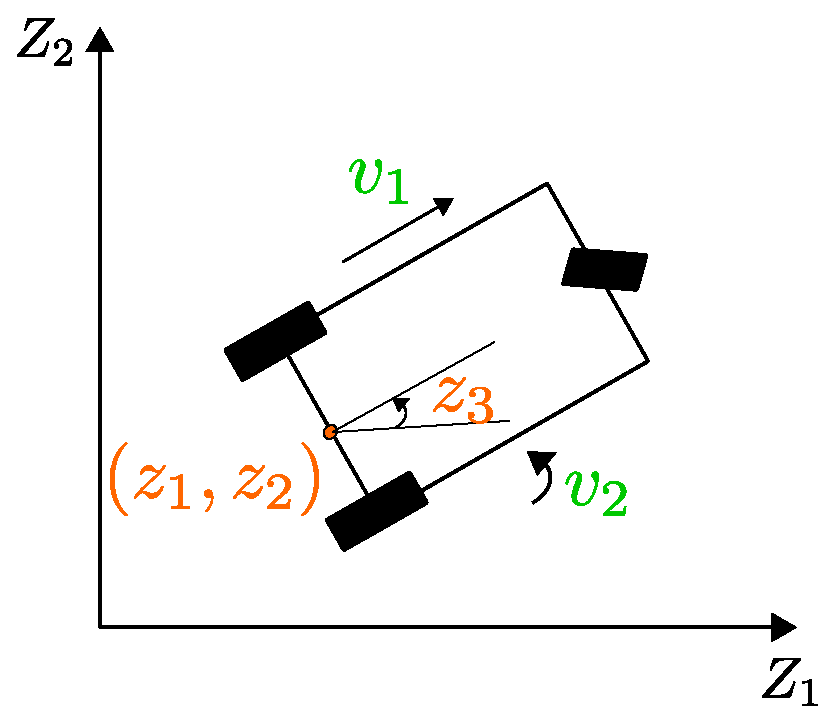
\includegraphics[width=0.4\linewidth]{bild/modul/Brocketts_Beispiel.eps}%6cm
		\caption[Skizze des mobilen Roboters mit einem Voreinrad.]{Skizze des mobilen Roboters mit einem Voreinrad. $(z_{1}, z_{2},z_{3})$ sind die Systemzustände und $(v_{1},v_{2})$ sind die Systemeingänge.}
		\label{fig:Brocketts_Doppelintegrator}
	\end{figure}  
	\begin{eqnarray}
	\dot{z}_{1} &=& v_{1}cos(z_{3})\notag\\
	\dot{z}_{2} &=& v_{1}sin(z_{3})\notag\\
	\dot{z}_{3} &=& v_{2}.
	\label{eq:Mobiler_Roboter_mit_Einrad}
	\end{eqnarray} 
	Das System hat $3$ Zustandskomponente: $z_{1}$ und $z_{2}$ steht jeweils für die Position des Punktes in der Mitte der der Hinterachse. $z_{3}$ ist der Winkel des Vorderrades mit der $z_{1}$-Achse. In dem System ergibt sich zwei Eingänge $v_{1}$ und $v_{2}$, die die Vorwärts- und Winkelgeschwindigkeit bedeuten.

	Mit der Rückkopplung der Systemzuständen und Eingängen \cite{liberzon2012switching}: 
	\begin{eqnarray}
	x_{1} &=& z_{1}\cos(z_{3}) + z_{2}\sin(z_{3})\notag\\
	x_{2} &=& z_{3}\notag\\
	x_{3} &=& 2\cdot(z_{1}\sin(z_{3})-z_{2}\cos(z_{3})) - z_{3}(z_{1}\cos(z_{3})+z_{2}\sin(z_{3}))\notag\\
	u_{1} &=& v_{2}\notag\\
	u_{2} &=& v_{1} - v_{2}(z_{1}\sin(z_{3})-z_{2}\cos(z_{3}))
	\label{eq:Mobiler_Roboter_mit_Einrad_Brockett_Doppelintegrator_Transformation}
	\end{eqnarray}
	kann Gln. \eqref{eq:Mobiler_Roboter_mit_Einrad} in der Form wie folgt transformiert werden:   
	\begin{eqnarray}
	\dot{x}_{1} &=& u_{1}\notag\\
	\dot{x}_{2} &=& u_{2}\notag\\
	\dot{x}_{3} &=& x_{2}u_{1}-x_{1}u_{2}.
	\label{eq:Brockett_Doppelintegrator}
	\end{eqnarray}
	Diese Zustandsfunktion beschreibt das berühmte System ``Brocketts nicht-holonomer Integrator''. 
  	Das Zustandsraummodell dieses Systems davon lautet:
	  \begin{eqnarray}
	  \dot{\vect{x}} = \begin{bmatrix}
	  0 & 0 & 0\\ 
	  0 & 0 & 0\\
	  -u_{2,e} & u_{1,e} & 0
	  \end{bmatrix}\vect{x} + \begin{bmatrix}
	  1 & 0\\
	  0 & 1\\
	  x_{2,e} & -x_{1,e} 
	  \end{bmatrix}\vect{u}
	  \label{eq:Brockett_doppel_Sytemzustand}
	  \end{eqnarray}
  	Ersetzt man den linken Teil von Gln. \eqref{eq:Brockett_doppel_Sytemzustand} mit $\vect{0}$, erhält man die Ruhelagen dieses Systems: $(x_{1},x_{2},x_{3})=(c_{1},c_{2},c_{3})$ beliebig mit $u_{1}=u_{2}=0$. Das heißt, die Eigenwerte des Systems sind alle $0$, \textbf{ohne} positive Realteile zu verfügen. Die Brockett $1.$ Bedingung ist nicht verletzt.
   
  	Zur Konstruktiven der $2.$ Bedingung kann man einen Regler wie folgt entwerfen:
	  \begin{eqnarray}
	  	\begin{pmatrix}
	  	0\\ 
	  	0\\ 
	  	0
	  	\end{pmatrix}\xrightarrow[Phase-\textrm{I}, 1s]{\vect{u}_{1}}\begin{pmatrix}
	  	\ast \\ 
	  	\ast \\ 
	  	0
	  	\end{pmatrix}\xrightarrow[Phase-\textrm{II}, 1s]{\vect{u}_{2}}\begin{pmatrix}
	  	\ast \\ 
	  	\ast \\ 
	  	\omega 
	  	\end{pmatrix}\xrightarrow[Phase-\textrm{III}, 1s]{\vect{u}_{3}}\begin{pmatrix}
	  	\alpha\\ 
	  	\beta\\ 
	  	\gamma
	  	\end{pmatrix}
	  \end{eqnarray}
  	mit $\vect{u}_{1}, \vect{u}_{2}, \vect{u}_{3}$ drei Regelgesetzen (nicht Regler $u_{1}$ oder $u_{2}$ in Gl. \eqref{eq:Brockett_Doppelintegrator}) in drei Phasen (Nimmt man an, dass jede Phase $1s$ dauert.) und $\begin{pmatrix}
   \ast  & \ast  & 0
   \end{pmatrix}^{T}, \begin{pmatrix}
   \ast  & \ast  & \omega
   \end{pmatrix}^{T}$ zwei Hilfspunkte. Es ist schon bekannt, wenn eine Trajektorie von Punkt A nach B existiert, gibt es unbedingt eine umgekehrte Trajektorie von B nach A. Ohne die Einfachheit zu verlieren, konstruiert man hier die Trajektorie von der Ursprung $(\vect{x}=\vect{0})$ nach einem beliebigen Punkt $(\vect{x}_{end}=(\alpha,\beta,\gamma))$.  In Phase-$\textrm{I}$ soll der Zustandsvektor mit $\vect{u}_{1}$ aus der Ruhelage zu den Hilfspunkt $1$ gehen, dann soll er in $1s$ zu den Hilfpunkt $2$ erreichen. Und endlich soll er mittels $\vect{u}_{3}$ am beliebigen Punkt $\begin{pmatrix}
   \alpha  & \beta  &\gamma
   \end{pmatrix}^{T}$ stoppen können. 
  
   EinAnsatz mit Konstanten $u_{1}$ und $u_{2}$ wie:
   \begin{eqnarray}
   Phase-\textrm{I}:~u_{1} = a_{1}, u_{2} = b_{1}\notag\\
   Phase-\textrm{II}:~u_{1} = a_{2}, u_{2} = b_{2}\notag\\
   Phase-\textrm{III}:~u_{1} = a_{3}, u_{2} = b_{3}
   \end{eqnarray}
   ist genügend, die obere Trajektorienbedingungen zu erfüllen.
   Zum Zeitpunkt $t=3s$ gilt:
   \begin{eqnarray}
   x_{1}(3s) &=& a_{1}  +a_{2} + a_{3}\notag\\
   x_{2}(3s) &=& b_{1} + b_{2} + b_{3}\notag\\
   x_{3}(3s) &=& (b_{1} + b_{2})a_{3} - (a_{1} + a_{2})b_{3} + b_{1}a_{2} - b_{2}a_{1}.
   \end{eqnarray}
   Mit diesem Regelgesetz kann das System in $3s$ irgendwo außerhalb dem Punkt $(\alpha=0,\beta=0,\gamma=0)^{T}$ ankommen. Um diesen Endzustand erreichen zu können, muss $\omega$ in Hilfspunkt $2$ äquivalent zu $\gamma$ sein. Das ist die einzelne Anforderung von der Größe von $(\alpha,\beta,\gamma)$. Deswegen kann das System mit diesem Regelgesetz die Brockett $2.$ Bedingung erfüllen.
  
   Letztlich wird die 3. Bedingung überprüft. Setzt man voraus, dass $\vect{\epsilon}$ in der offenen Menge $M=B(\vect{x},\varepsilon)$ liegt, dann gilt 
   \begin{eqnarray}
   \vect{\epsilon}  = \begin{bmatrix}
   \epsilon _{1}\\ \epsilon_{2} \\ \epsilon_{3}
   \end{bmatrix} = 
   \begin{bmatrix}
   u_{1\epsilon }\\ u_{2\epsilon } \\ x_{2\epsilon}u_{1\epsilon}- x_{1\epsilon}u_{2\epsilon}
   \end{bmatrix}.
   \label{eq:doppel_Brockett}
   \end{eqnarray}
  
   Die Menge $M$ enthält einen Punkt $\vect{x}_{um}=(0,0,\delta)$ mit $\delta<\varepsilon$. Offensichtlich ist es unmöglich, das Bild der Abbildung $\Gamma: \left ( \vect{x},u \right ) \mapsto \vect{f}\left ( \vect{x},u \right )$ einen Wert gleich $\vect{x}_{um}$ zu sein. Nämlich ist $\Gamma$ nicht surjektiv zu $M$.
  
   D.h. das System verletzt die Brockett Bedingung. Deswegen existiert kein stetig differenzierbarer Regelgesetz, mit dem der Ursprung asymptotisch stabil ist.
\end{beispiel}
 
Fazit: In diesem Kapitel wurde das Brockett Theorem für die Überprüfung der Existenz einer asymptotischen stabilen Ruhelage in einem nichtlinearen System mittels eines stetigen differenzierbaren Regelgesetz vorgestellt. In den Literatur \cite{brockett1983asymptotic} lieferte Brockett schon einen Beweis für das Theorem, der aber für die Leser ohne tiefen Kenntnisse der Topologie  vergleichsweise schwer verständlich ist. Daher erklärt die Autorin hier den Beweisvorgang mit einfacheren Worten. Ein einfaches nichtholonom Doppelintegrator System wurde als Beispiel für die Anwendung der Brockett-Bedingung diskutiert.